\documentclass[fleqn]{article}

\usepackage{amsmath, amsthm, amssymb}
\usepackage{geometry}
\geometry{margin = 3.0 cm}

\usepackage{enumerate}
\usepackage{url}
\usepackage{listings}
\usepackage{color}

\usepackage{float}
\usepackage{graphicx}
\usepackage{subfigure}

\usepackage{tikz}
\usetikzlibrary{shapes}
\usetikzlibrary{arrows}
\usetikzlibrary{calc}

\tikzset{node distance=2cm, auto}
 
\definecolor{lightergray}{RGB}{230,230,230}

%\usepackage{alg}
\usepackage{caption}
%\usepackage{algpseudocode}
%\algblockdefx[NAME]{Input}{EndInput}
%    [1][]{\textbf{Input:} #1}
%    {}
%
%\algblockdefx[NAME]{Output}{EndOutput}
%    [1][]{\textbf{Output:} #1}
%    {}

%\newcommand{\myalg}[2]{\begin{figure}[H]
%    { \renewcommand{\figurename}{Algorithm}
%\begin{center}
%\begin{minipage}{0.6\textwidth}
%\hrulefill
%\begin{algorithmic}[1]
%    #1
%\end{algorithmic}
%\hrulefill
%\end{minipage}
%\end{center}
%\caption{#2}
%}
%\end{figure}}

\renewcommand{\l}{\lambda}
\renewcommand{\L}{\Lambda}
\renewcommand{\mod}{~\mathrm{mod}~}
\renewcommand{\div}{~\mathrm{div}~}

\renewcommand{\vec}[1]{\mathbf{#1}}

\renewcommand{\(}{\left(}
\renewcommand{\)}{\right)}

\newcommand{\dist}{\text{dist}}
\newcommand{\todo}[1]{\textcolor{red}{#1}}

\newcommand{\mat}[1]{\begin{pmatrix} #1 \end{pmatrix}}
\newcommand{\room}{\hspace{0.5cm}}
\newcommand{\hl}[1]{\textbf{#1}}
\newcommand{\ceil}[1]{\lceil #1 \rceil}
\newcommand{\floor}[1]{\lfloor #1 \rfloor}

\newcommand{\tm}{\textsuperscript{\texttrademark}}
%\def\tm{$^{\hbox{\tiny TM}}$~}
%\renewcommand{\tm}{ }

\newtheorem{lem}{Lemma}

\usepackage{tikz} \usetikzlibrary{shapes}
\usetikzlibrary{arrows}

\tikzset{node distance=3cm, auto}

\lstset{language=C++,
                basicstyle=\ttfamily,
                keywordstyle=\color{blue}\ttfamily,
                stringstyle=\color{red}\ttfamily,
                commentstyle=\color{green}\ttfamily,
                morecomment=[l][\color{magenta}]{\#}
}

\title{\textsc{Implementation of the BSP model for the Epiphany\tm architecture}}
\author{Jan-Willem Buurlage \ Abe Wits \\ \normalsize{Utrecht University, The Netherlands}}

\begin{document}

\maketitle

\abstract{In this report we introduce the \texttt{epiphany-bsp} library, an implementation of the BSP model on the Epiphany\tm architecture. This library is inteded as an alternative for the Epiphany SDK with minimal overhead, and should allow for easy ports BSP programs to this architecure. In this report we will first give an introduction to the Epiphany architecture, and we give some technical details of current hardware that ship with an Epiphany\tm chip. Next we describe the BSP library that we developed, and will briefly touch on various implementation details. We will also provide some examples and use cases of the library, and present some early measurements of its performance. Finally we will discuss features we have planned for the future, as well as propose some platform-specific extensions to the BSP library.}

\newpage

\tableofcontents

\newpage

\setlength{\parskip}{0.2 cm}
\setlength{\parindent}{0.0 cm}
\setlength{\mathindent}{1.0 cm}

\section{Introduction}

The Epiphany\tm architecture is a multi-core microprocessor architecture that was developed by Adapteva\footnote{\url{http://www.adapteva.com}}. The Epiphany\tm architecture is implemented on chips that are inteded as a coprocessor to ARM/Intel CPUs. Every core has access to local, and shared memory. Besides the Epiphany\tm technology Adapteva has developed the Parallella board\footnote{\url{http://www.parallella.org}}, which is a computer with the size of a credit card that is based on this multi-core coprocessor technology. Although the architecture was initially designed for embedded real time signal processing applications, it has also gained interest from the High Performance Computing community because of its energy-efficiency and scalability \cite{ep:whitepaper}.

There are already some popular parallel-programming paradigms are available for this architecture, e.g. OpenCL and lightweight versions of MPI and OpenMP. However, in our experience, because of the limited on-core memory, currently the only feasible way to program this architecture is by using the supplied software development kit, the Epiphany SDK (ESDK). In our opinion the ESDK lacks proper documentation, and is not particularly inviting for people new to the EA. It is also undergoing heavy changes in every iteration, and some commonly requested features are in the work.

In this report we describe a new library for the EA, which is built on top of the ESDK called Epiphany-BSP. The Bulk Synchronous Parallel (BSP) computing model is a model for designing parallel algorithms. It provides a description of how parallel computation should be carried out. Programs written with this model consist of a number of supersteps, which in turn consist of local computations and non-blocking communication. A (barrier) synchronisation at the end of such a step is used to guarantee occurance of all communications within a step. We will describe the BSP model in some more detail in the next section. 

The major benefit of the BSP model and its implementations is that it has a straightforward paternalistic interface for developing BSP programs and algorithms. This means in particular that programs developed with this model will not differ from platform to platform, and in the particular case of the EA between different iterations of the ESDK, since we are able to make the necessary changes in the implementation of the library itself. Later in this report we will introduce the Epiphany architecture and present some technical details on the intented target hardware.

\section{The Bulk Synchronous Parallel model}

The Bulk Synchronous Parallel (BSP) model was developed by Leslie Valiant in the 1980s. It was introduced in an article in 1990 \cite{bsp:valiant}. The BSP model is intended as a bridging model between parallel hardware and software. It is an elegant and simple model that has a small and easy to understand interface.

The BSP model is defined on an abstract computer called a BSP computer. This computer has three important requirements.
\begin{enumerate}[1.]
\item It has $n$ processors capable of computation and communication, i.e.\ it allows for local memory transactions.
\item It has a network in place that allows the different processors to send and receive data.
\item It has a mechanism that allows for the synchronisation of these processors, e.g.\ by means of a blocking barrier.
\end{enumerate}

A BSP program consists of a number of distinct blocks of computation and communication called \emph{supersteps}. These steps are separated by a barrier synchronisation, and consist of a \emph{computation} and a \emph{communication} step.

An important part of a BSP algorithm is the associated cost function. To this end we introduce two important concepts: namely an $h$-relation, and a notion of the work done by a processor. Furthermore we introduce two parameters that define a BSP computer: $g$ and $l$.

An $h$-relation is a superstep in which each processor sends or receives a maximum of $h$ words of data.We commonly denote with $p$ the id of a processor such that we can write for the $h$-relation:
$$h = \max_{p} ~ \max \{ (h_p)_\text{sent} ,  (h_p)_\text{received} \}$$
Where $h_p$ denotes the number of words received or sent by processor $p$. Similarly we define the work $w$ done in a superstep as the maximum number of flops (\emph{flo}ating \emph{p}oint operation\emph{s})  performed by all processors. Finally we define the \emph{latency} $l$ of a superstep as the fixed constant overhead, used primarily to account for the barrier synchronisation. The values for $g$ and $l$ are computer-specific constants that are found emperically. The values for $w$ and $h$ are superstep specific and commonly obtained analytically. The total cost of a BSP algorithm is then:
$$ \sum_{i \in \text{supersteps}} \( w_i + g h_i + l \)$$

The BSP model has gained significant interest in the last couple of years. Most notably because Google has adopted the model and has developed some technologies based on BSP such as MapReduce \cite{goo:mapreduce} and Pregel \cite{goo:pregel}. The standard for BSP implementations is BSPlib\footnote{\url{http://bsp-worldwide}} which will be discussed in more detail when we introduce the library later in this report. Modern implementations of the BSP model include BSPonMPI \cite{bsponmpi}, which simulates the BSP model on top of MPI, and MulticoreBSP \cite{multicorebsp} which provides a BSP implementation for shared-memory multi-core computers.

For a more detailed introduction on the BSP model, as well as a large number of examples of BSP programs we refer to the introductory text by Rob Bisseling \cite{bsp:bisseling}.

\section{The Epiphany\tm architecture}

The Epiphany\tm architecture (EA) consists of a number of Reduced Instruction Set Computer (RISC) cores, and is currently defined for 1-4096 cores. These cores have a certain amount of local on-core memory and are part of a multi-core framework. There is a Network-On-Chip (NOC) present, designed for real time applications. This allows the different cores and the host processor, to communicate with eachother. 

\subsection{Memory model}

The local memory on the EA uses an adress space that consists of $2^{32}$ bytes \cite{ep:sdkdoc}. Following the documentation we will call this the \emph{global address space}. Besides this each Epiphany core has an aliased range of local addresses. Current models have 32KB of local memory per chip, which starts at \texttt{0x0000} and ends at \texttt{0x7FFF}. This space is partitioned in 4 memory banks starting at \texttt{0x0000}, \texttt{0x2000}, \texttt{0x4000}, and \texttt{0x6000}. Furthermore, there are registers available at \texttt{0xF0000}, and the space between the banks and the register space as well as the space after the registers is reserved. This address space is referred to as \emph{local address space}.

\begin{figure}[H]
\centering
\begin{subfigure}
\centering
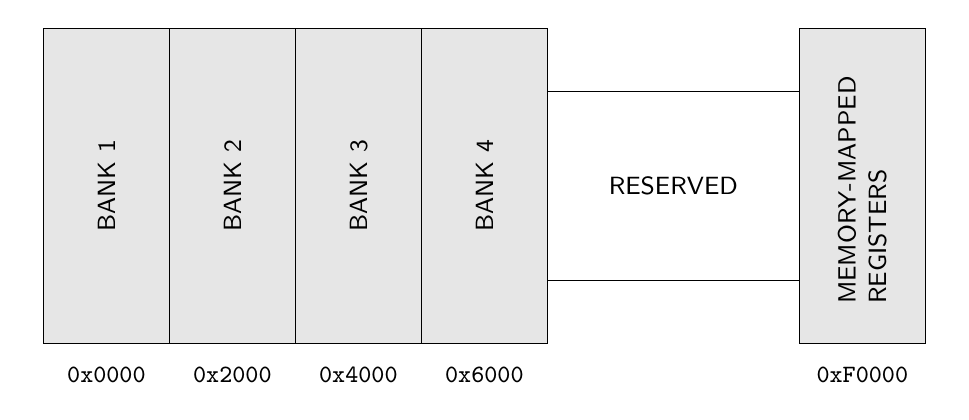
\begin{tikzpicture}[scale=0.8,font=\sffamily\small]
\tikzset{node distance=2cm, auto}
\filldraw[fill=lightergray, draw=black] (0, 0) rectangle (2, 5);
\filldraw[fill=lightergray, draw=black] (2, 0) rectangle (4, 5);
\filldraw[fill=lightergray, draw=black] (4, 0) rectangle (6, 5);
\filldraw[fill=lightergray, draw=black] (6, 0) rectangle (8, 5);
\filldraw[fill=white, draw=black] (8, 1) rectangle (12, 4);
\filldraw[fill=lightergray, draw=black] (12, 0) rectangle (14, 5);

\node[minimum width=2cm,font=\sffamily\small] at (1, -0.5) {\texttt{0x0000}};
\node[minimum width=2cm,font=\sffamily\small] at (3, -0.5) {\texttt{0x2000}};
\node[minimum width=2cm,font=\sffamily\small] at (5, -0.5) {\texttt{0x4000}};
\node[minimum width=2cm,font=\sffamily\small] at (7, -0.5) {\texttt{0x6000}};
\node[minimum width=2cm,font=\sffamily\small] at (13, -0.5) {\texttt{0xF0000}};
\node[minimum width=2cm,rotate=90] at (1, 2.5) {BANK 1};
\node[minimum width=2cm,rotate=90] at (3, 2.5) {BANK 2};
\node[minimum width=2cm,rotate=90] at (5, 2.5) {BANK 3};
\node[minimum width=2cm,rotate=90] at (7, 2.5) {BANK 4};
\node[minimum width=2cm, text width=3cm, rotate=90] at (13, 2.5) {MEMORY-MAPPED REGISTERS};
\node[minimum width=2cm] at (10, 2.5) {RESERVED};

\end{tikzpicture}
\end{subfigure}
\caption{The local address space corresponding to a single Epiphany core. This figure has been adapted from Figure 1.2 in \cite{ep:sdkdoc}}
\label{fig:localspace}
\end{figure}




The memory is freely accessible and one can choose where to store the data and code (i.e.\ parts of the binary), however it is best for performance to use separate banks for data and code. To achieve this one currently has to use linker scripts in order to explicitely place data and code \cite{ep:sdkdoc}. However, more convenient methods are planned for future SDK releases. There is also an interface available for setting the memory-mapped registers. For a complete overview of these registers we refer to \cite{ep:archdoc}.

\subsection{Epiphany\tm Efficiency}
The 16-core Epiphany-III\tm can do roughly 5.0 GFLOPs/W, the 64 core Epiphany-IV\tm can do 50 GFLOPs/W (both single precision). This makes the 64-core Epiphany-IV\tm chip one of the most energy efficient processors currently available \cite{ep:power}. The most efficient supercomputer can do only 3.0 GFLOPs/W. However, the total amount of GFLOPs is relatively low. Adapteva (the developing company) claims that the techniques used are scalable, and more powerful chips with comparable power consumption are developed. If Adapteva can deliver on its promises, Epiphany\tm chips could play a role in embedded systems; for example drones, phones or tablets. It could, for example, make advanced image processing possible in mobile devices for a wide array of applications.


\section{Parallella Board}

The Parallella board was introduced by Adapteva in a Kickstarter\footnote{Kickstarter is a crowd-funding website. See \url{http://www.kickstarter.com} for more information} campaign. Inspired by projects such as the Arduino and the Raspberry Pi, the Parallella is a credit-sized computer that is designed to be energy-efficient, and to have high-performance \cite{par:manual}. Besides this, both the board design and the available software, are completely open source. In this section we will provide a short introduction to the capabilities of the board from a High Performance Computing (HPS) point-of-view. This means that we will focus on the processors and the different types of memory that are involved, and refer to the documentation for details on the peripherals (USB, HDMI, GPIO, SD Card, etc.) which are particularly of interest for hardware projects. 

The original Parallella boards consist of a Zynq-7000 series Dual Core ARM processor, a 16 or 64 core Epiphany processor and has 1GB of SDRAM available. The 16 core variant is available in high volume, while the Parallella with a 64 core Epiphany processor has so far only been available in very limited quantities. Below we present a schematic overview of the Parallella board, and some useful facts about the ARM and Epiphany-III processor.

\begin{table}[h]
\centering
\begin{tabular}{l|ll}
& Host & Coprocessor \\
\hline
Processor type & ARM & Epiphany-III\tm \\
Scope & Global & Local \\
Library & eHAL & eLib \\
Memory & 1 GB & 32 KB \\
\# of cores & 2 & 16 \\
Clock speed & 677 MHz & 600 MHz\\

\end{tabular}
\caption{Some useful facts about the Parallella board}
\end{table}


\begin{figure}[H]
\centering
\begin{subfigure}
\centering
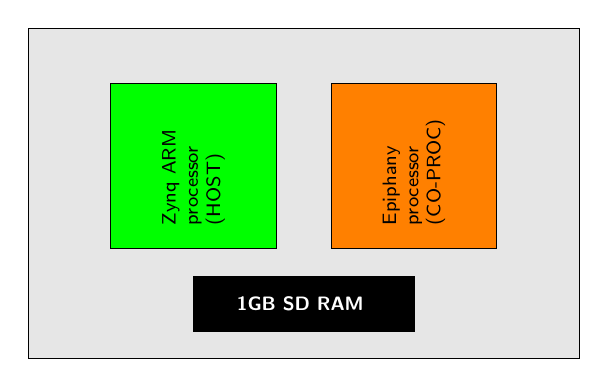
\begin{tikzpicture}[scale=0.7,font=\sffamily\scriptsize]
\tikzset{node distance=2cm, auto}
\filldraw[fill=lightergray, draw=black] (0, 0) rectangle (10, 6);
\filldraw[fill=green, draw=black] (1.5, 2.0) rectangle (4.5, 5.0);
\filldraw[fill=orange, draw=black] (5.5, 2.0) rectangle (8.5, 5.0);
\filldraw[fill=black, draw=black] (3.0, 0.5) rectangle (7.0, 1.5);
\node[minimum width=1.5cm, text width=1.5cm, rotate=90] at (3, 3.5) {Zynq ARM processor (HOST)};
\node[minimum width=1.5cm, text width=1.5cm, rotate=90] at (7, 3.5) {Epiphany processor (CO-PROC)};
\node[minimum width=3.0cm, text width=1.7cm] at (5, 1.0) {\textbf{\textcolor{white}{1GB SD RAM}}};
\end{tikzpicture}
\end{subfigure}
\caption{A simple schematic showing the processor- and memory structure of the Parallella board.}
\label{fig:localspace}
\end{figure}


The Parallella board runs Ubuntu and is programmable through the Parallella SDK.
\subsection{Memory}
Note that only a very small amount of memory is available locally! This small local cache also contains the executable, leaving little memory for our algorithm; the Hello World implementation provided by Adapteva has a binary of 14KB, that is more than 40 percent of the memory available locally. The global memory can be used to store larger variables, but doing this in an efficient way is non-trivial and does not adhere to the BSP-model. One possible way to use bigger programs is to split it into several smaller programs, leaving supersteps intact. The cost of loading a new program image could be seen as additional synchronisation cost, increasing $l$.

Direct communication between cores is essential to the BSP model; if all communication has to go through the ARM processors and/or local memory, the central assumption that communication speed is determined by the largest amount of data sent/received by one processor breaks down. Instead we would get (semi)linear behaviour, reducing the advantages of parallel computing. Also, efficient usage of the Parallella board would require thoughtful modification of the regular optimal BSP-algorithms. 


\section{BSP on Epiphany\tm}

Implementing the BSP library on the Epiphany\tm architecture comes with a number of challenges. We are dealing with a very different situation from common systems, in that there is a host processor, and a coprocessor. Not only is there a hierarchy in processors, but we are also dealing with two kinds of memory. We have the cache, local to the cores on the Epiphany chip, and the shared memory. In the next section we will describe the choices we have made for the various components of the BSP system, and describe in turn each BSP primitive and the specifics of their implementations.

\subsection{Design choices}

The nature of the Epiphany\tm architecture is such that in order to run programs on the Epiphany cores we have to do some initial work on the host processor. We therefore make the decision to divide our BSP programs in two parts. Part (1), the \textbf{host part} runs on the host processor, and is responsibly for setting up the Epiphany system, loading and starting the Epiphany binary, initializing and distributing memory and data, and all the sequential parts at the end of the program (e.g.\ presenting data). Furthermore we use the host-processor as a middle-man in barrier synchronisations, in particular for registering variables. The actual work of the algorithm is done in part (2), the \textbf{coprocessor part}, which describes a program in the traditional SPMD (single program multiple data) style of the BSP model. Note that this separation in two parts implies that already written BSP will have to undergo some modifications before they can run on this new platform, but we have designed the library to keep these modifications as minimal, in both number and size, as possible.

A program in part (1) starts with distributing the data over the cores. For this we have written a convenient routine \verb%ebsp_write% which allows communication from the host to the coprocessor in a BSP-styled fashion. Next we initialize the BSP system, and begin running the SPMD part on a given number of cores. For the core numbering we rely on the workgroup style as defined by the Epiphany\tm SDK, and the processor identifiers will also be provided to the program run on the coprocessor. Next we start the part (2) program, which is a program that runs on the Epiphany\tm architecture. After all the cores have finished, we end the BSP program by running a sequential part to analyze the result (using \verb%ebsp_read% to retrieve the memory on the cores) and finally we clean and reset the system.

The SPMD program in part (2) will not differ much from their counterparts in the traditional BSP libraries. Here the user has access to all the BSP primitives, as if we would be writing in any other platform. This is precisely the power of the BSP model.

\subsection{Variable registration}

First we will present how variable registration works in BSP:
\begin{lstlisting}
void bsp_push_reg (const void *ident, int size);
void bsp_put(int pid,const void *src,void *dst,int offset,int nbytes);
\end{lstlisting}
Above are the BSP commands to register a variable and to put some value in a registered variable.
All processors have to register a variable in the same superstep. BSP will ``tie together'' the pointers passed in \texttt{bsp\_push\_reg}; they are assumed to all point to a local version of the same variable. We will give this set of variables an index, \texttt{slotID}. Then if we use \texttt{bsp\_put}, we pass a local pointer \texttt{*dst} and a \texttt{\texttt{pid}}; they form an adress to the local version of \texttt{*dst} in processor \texttt{pid}. To be able to give this adress, we need some mapping of \texttt{*dst} to all the pointers with the same \texttt{slotID}; this implies they were registered in the same superstep. Then we need to take the pointer that is local to processor \texttt{pid}.

If a normal (non-tiny) amount of memory is available, we could for example write the required data structures in C++ like this:
\begin{lstlisting}
map<void*, int> pointer_to_slotID;
vector<vector<int> > registered_variables;
\end{lstlisting}
Given \texttt{*dst} and \texttt{pid}, we can now give the actual pointer to the version of \texttt{*dst} local to processor \texttt{pid}:
\begin{lstlisting}
int slotID = pointer_to_slotID[dst];
void* actual_destination=registered_variables[slotID][pid];
\end{lstlisting}
With this approach, we need only $\mathcal{O}(\log(n))$ time to get the correct \texttt{slotID}, and we can then get \texttt{actual\_destination} in $\mathcal{O}(1)$ time. The std::map and std::vector datastructures are of variable size and allow fast insertion. However, they do have some memory-overhead; std::map is implemented as a red-black tree, and needs $48+(32+size)*length$ bytes (in GNU 64 bit C++ library), $size$ is of order 8 bytes (\texttt{sizeof(void*)+sizeof(int)}). When we register 10 variables, the map will use ~500 bytes. A vector uses approximately $24+size*length*2$ bytes, our vector of vectors will use order 4KB if we use 16 processors and we register 10 variables. To put this in perspective; on our Epiphany this map and vector use respectively 2 and 13 percent of the available memory!

Instead we use only one datastructure:
\begin{lstlisting}
void** registermap;
\end{lstlisting}
\texttt{registermap[slotID*nProcs+pid]} is the pointer to the \texttt{slotID}th variable in processor pid.
We get the correct \texttt{slotID} by finding \texttt{*dst} among all variables registered by our current processor, this takes $\mathcal{O}(n)$ time, but since it is very likely that $n$ is small, this is acceptable. It is not as flexible; to resize we need to allocate new memory, this is relatively expensive and clumbsy in such small memory. However, the number of variables that has to be registered is usually known beforehand. This is the only structure we need, and it uses only 640 bytes for 16 processors and 10 registered variables.

\subsection{Primitives}

All BSP implementations expose a number of public function used as an interface to the BSP system. These functions are called \emph{primitives}. A minimal BSP implementation requires as little as 8 primitives. In this section we will introduce the different BSP primitives that were implemented for the Epiphany BSP (EBSP) library that we developed.

\subsubsection{On the host processor}

The first BSP primitive that is called in any BSP program is \verb%bsp_init%. It has the following form:
\begin{equation}
    \verb.bsp_init(const char* e_program_name, int argc, char** argv).
\end{equation}
    Here, \verb%e_program_name% is the name given to the Epiphany\tm program, and the other two arguments pass along the input arguments to our program. In this initial version of the library the latter arguments are ignored, but are passed for the sake of portability. This function will first initialize the Epiphany system for working with the host processor and reset the system, and next obtain information on the system and initialize and store the state of the BSP system.

After the system is initialized, we can indicate the start of the BSP program by passing the number of cores we want to use to the following primitive:
\begin{equation}
    \verb.bsp_begin(int nprocs). 
\end{equation}
This will make the necessary workgroups\footnote{The ESDK requires the initialization of a number of cores in a so called workgroup. A workgroup is indicated by an offset an a size, e.g. a 16 core Epiphany processor has its cores laid out in a $4 \times 4$ grid and the workgroup with offset $(1, 1)$ and size $(2, 2)$ would select the cores in the interior}, load the Epiphany binary to the cores, and initialize the BSP system on the coprocessor.

Since we define the SPMD part for the Epiphany processor, we have made an auxilliary function that starts their execution cllaed \verb.ebsp_spmd().. This function will return when all the cores on the Epiphany chip have finished executing the parallel part of the program. 

The end of the program on the host processor is indicated by the primitive:
\begin{equation}
    \verb.bsp_end(). 
\end{equation}
Before calling this primitive a sequential part can be run on the host processor to gather and present the obtained results.

The last primitive that is available on the host processor allows the user to obtain the number of available cores. 
\begin{equation}
    \verb.bsp_nprocs(). 
\end{equation}
For numbering the cores we try to follow the layout that is given to us by the ESDK, but since we allow for the BSP program to be run on an arbitrary number of processors we might need multiple (square) workgroups to work around the limitations of the ESDK. After \verb.bsp_begin(). is called this primitive will return the number of cores in use, instead of the total number of cores available such that we can use it for data-retrieval.

\subsubsection{On the coprocessor}

In the SPMD program on the Epiphany processor we have two BSP primitives that can be used to gather general information about the system. Similar to the host processor we have access to the number of cores through the function:
\begin{equation}
    \verb.bsp_nprocs(). 
\end{equation}
Which on the coprocessor always returns the number of cores in use instead of the number of cores that are available. Furthermore we have access to our processor id (which in the case of EBSP is our core number) $p$ by the primitive:
\begin{equation}
    \verb.bsp_pid(). 
\end{equation}
Now we come to a very important and non-trivial component of the BSP system, namely memory management and data transfer. We will start by introducting three primitives that are required to construct a fully functioning BSP program.

If we want to share data with another core, we first have to define a common variable name. This variable is defined in every core (since the program is written in a SPMD style) but can have a different size on different cores.  A variable is registered with the primitive:
\begin{equation}
    \verb.bsp_push_reg(const void* variable, const int nbytes). 
\end{equation}
The first argument represents the location where the variable is stored, and the second argument indicates the size of the variable in bytes. Every single registration should be followed by a barrier synchronisation (see \verb.bsp_sync. below).

We can write to a variable on another core at any point in a superstep using the following two primitives:
\begin{equation}\verb.bsp_put(int pid, const void* src, void* dst, int offset, int nbytes).\end{equation}
\begin{equation}\verb.bsp_hpput(int pid, const void* src, void* dst, int offset, int nbytes).\end{equation}
The first argument represents the processor id of the receiving processor, the second argument defines the location of the data that is to be written, the third argument is the location of the (registered) variable to write to, and the last two arguments define the offset (relative to the location of the variable written to) and the number of bytes to write. The first of these primitives \verb.bsp_put. is buffered, and will only be resolved at the end of every superstep, whereas the second primitive \verb.bsp_hpput. (which stands for high-performance put) is an unbuffered variant which is resolved immediately.

The final primitive we will discuss here performs the barrier synchronisation that indicates the end of every superstep, and is called without any arguments.
\begin{equation}
    \verb.bsp_sync(). 
\end{equation}
Other primitives will be added to the library over time.

\subsection{An example of a BSP program}

A minimal BSP program on the host processor has the following form:
\begin{lstlisting}[numbers = left]
#include <host_bsp.h>

int main() {
    bsp_init("e_program.srec", argc, argv);
    bsp_begin(bsp_nprocs());
    ebsp_spmd();
    bsp_end();

    return 0;
}
\end{lstlisting}
This will run the Epiphany binary \verb.e_program. on all available Epiphany cores. The code for the Epiphany binary begins with initializing the system, e.g.\
\begin{lstlisting}[numbers = left]
#include <e_bsp.h>

int main() {
    // initialize the BSP system
    bsp_begin();
    int n = bsp_nprocs();
    int p = bsp_pid();

    // write the number of processors to a specific memory position
    int* a = (int*)0x2000;
    (*a) = p;

    // register a variable
    bsp_push_reg(a, sizeof(int));
    bsp_sync();

    // write our processor number to the `next' core
    bsp_put((p + 1) % n, a, a, 0, sizeof(int));
    bsp_sync();

    // finalize the BSP system
    bsp_end();

    return 0;
}
\end{lstlisting}
\section{Performance Measurements}
We ported BSP-bench (from BSPedupack) to do measurements of $g$ and $l$ on the Epiphany chip. Only some minor changes were required, mainly in memory management (replacing vecallocd and limiting the size of variables on the stack) and splitting code in some boilerplate on the ARM and the actual computations on Epiphany.

\subsection{BSP parameters / benchmark}
BSP-bench uses roughly $6*\mathtt{MAXH}+3*\mathtt{MAXN}$ floats, while there is room for about 2048 single precision floating point numbers. Because of this, we had to limit the size of $\mathtt{MAXH}$ and $\mathtt{MAXN}$. All measurements were taken using all 16 Epiphany cores.

\begin{table}[h]
\centering
\begin{tabular}{rrr|rrrrr}
$\mathtt{MAXH}$ & $\mathtt{MAXN}$ & $\mathtt{NITER}$ & $r$ (Mflop/s) & $g$ & $l$ & $g_0$ & $l_0$ \\
\hline
256 & 128 & 100 & 4.248 & 229 & 10121 & 242 & 16992 \\
128 & 256 & 100 & 5.008 & 284 & 10476 &  77 & 18890 \\
128 & 256 & 100 & 4.611 & 262 &  9665 &  77 & 17356 \\
 64 & 256 & 100 & 4.146 & 234 &  8758 & 276 & 15668 \\
 64 & 256 & 100 & 4.095 & 247 &  8954 &  29 & 16375 \\
\end{tabular}
\caption{The results of BSP-bench measurements\\ $g$, $l$, $g_0$ and $l_0$ are time in flop units of communication and synchronisation.}
\end{table}

The values measured are consistent. The values of $g$ and $l$ are plausible, but $r$ is very low; a floating point operation has to take 100 clock cycles to get 5 Mflop/s on a chip with 600 MHz, this is an order of magnitude too high. Communication on Epiphany seems to have strange behavior as well; take a look at Figure \ref{fig:bspbench}. The time needed to sent a package jumps if $h$ increases by 57 words. One possible explanation is that the Epiphany architecture sends data in a fixed time communication phase.

\begin{centering}
\begin{figure}[h!]
\centering
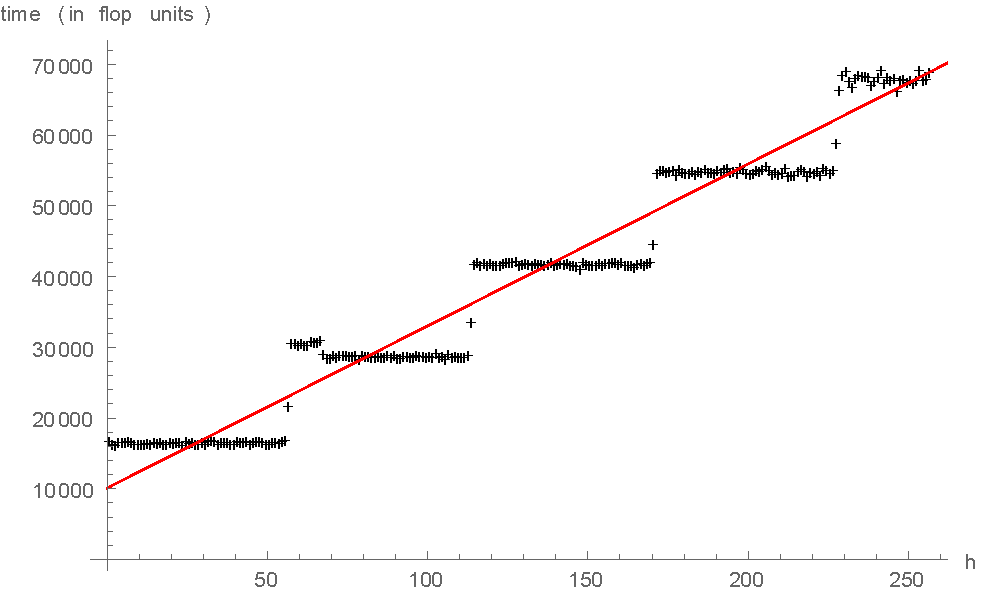
\includegraphics[scale=0.8]{EpiphanyGandL.pdf}
\caption{The time needed to sent packages of different size}
\label{fig:bspbench}
\end{figure}
\end{centering}


\section{Further Work}

In this section we summarize some of the ideas we are exploring for future releases of the library

\begin{itemize}
\item One of the major drawbacks of using the Epiphany architecture in its current state, specifically for high-performance computing purposes, is the limited amount of on-core memory that is available. In the current state of the library we can only safely use a single memory bank (depending on the stack- and binary size) freely, which means we only have 8 kb of local memory which leaves very room to work with. In order to work with larger amounts of data we want to let the host and coprocessor work together by introducing a function \verb.ebsp_next_chunk(). which swaps out the current set of data with the next such that we can utilize the speed of the local cache without resorting to the (slower) SDRAM because of memory-size limitations.
\item The SDRAM is currently not fully used by our library, we want to implement support for registering variables on the SDRAM and writing/reading to them with the corresponding primitives.
\item The ESDK has support for workgroups on different Epiphany chips. It should be possible to use this to make BSP programs that run simultaneously on different Epiphany computers such as multiple Parallella boards. This would require some significant additions to the communication system of the library. Some initial work using MPI has already been done. See for example: \url{http://www.adapteva.com/white-papers/building\-the-worlds-first-parallella-beowulf-cluster/}
\item The set of primitives our library supports in this initial release is rather limited, we want to add the other primitives defined by the BSPlib standard over time.
\end{itemize}


\section*{Appendix: Notes on installing EBSP}

The library has been tested with the 2014.11 version of the ESDK. Details for installing the SDK can be found on the Wiki for the GitHub project \verb.adapteva/epiphany-sdk.. The entire source code for the EBSP, as well as details required for installation can be found on the GitHub page \verb.buurlage-wits/epiphany-bsp..

\begin{thebibliography}{9}

\bibitem{ep:whitepaper}
  Kickstarting High-performance Energy-efficient Manycore Architectures with Epiphany

\bibitem{ep:sdkdoc}
  Epiphany SDK Reference

\bibitem{ep:archdoc}
  Epiphany Architecture Reference

\bibitem{par:manual}
  Parallella User Manual

\bibitem{bsp:valiant}
    Leslie G. Valiant, A bridging model for parallel computation, Communications of the ACM, Volume 33 Issue 8, Aug. 1990

\bibitem{bsp:bisseling}
    Parallel Scientific Computing. A structured approach using BSP and MPI. Prof. Rob H. Bisseling, Utrecht University. Oxford University Press.

\bibitem{ep:power}
    Vincent Hindriksen, Processors that can do 20+ GFLOPS per Watt, http://streamcomputing.eu/blog/2012-08-27/processors-that-can-do-20-gflops-watt/


\end{thebibliography}

\end{document}
